\begin{center}
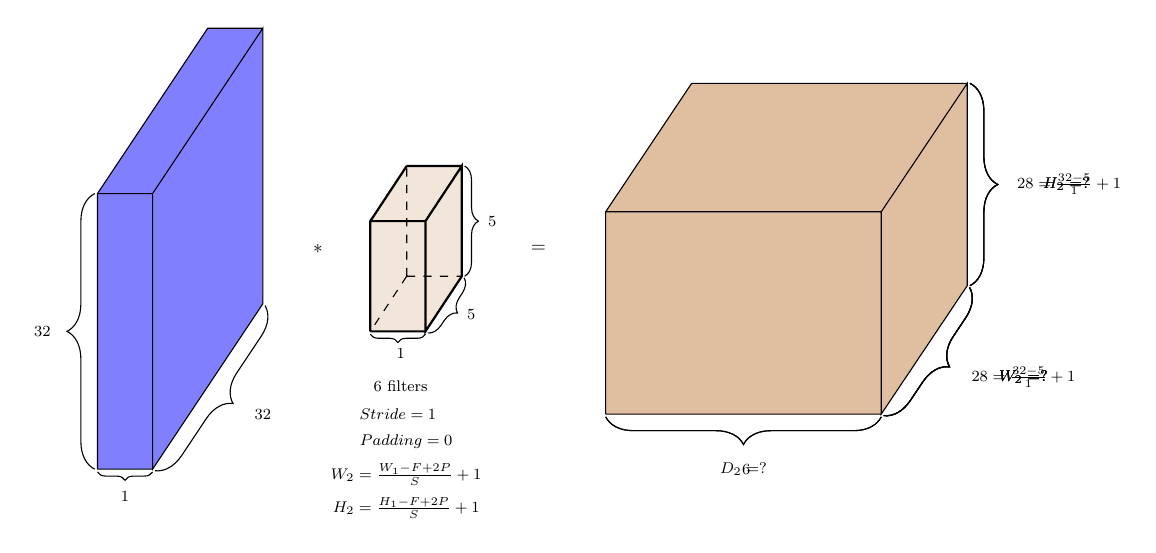
\begin{tikzpicture}[scale=0.7, transform shape]
\def\h{5}
\def\w{2}
\def\d{3}
\coordinate (A) at (0,0);
\coordinate (B) at (0,\h);
\coordinate (C) at (\w,\h+\d);
\coordinate (D) at (\w,\d);


\coordinate (A1) at (0+1,0);
\coordinate (B1) at (0+1,\h);
\coordinate (C1) at (\w+1,\h+\d);
\coordinate (D1) at (\w+1,\d);

\fill [draw=none, fill=blue!50] (A) -- (B) -- (C) -- (C1) -- (D1) -- (A1) -- cycle;
\draw (A) -- (B) -- (C) (A) -- (A1) (B) -- (B1) (C) -- (C1) (A1) -- (B1) -- (C1) -- (D1) -- cycle;

\draw [decorate,decoration={brace,amplitude=10pt,raise=1pt},xshift=0pt,yshift=0pt] (A) -- (B) node [black,midway,xshift=-1cm] {\footnotesize $32$};

\draw [decorate,decoration={brace,amplitude=3pt,raise=1pt},xshift=-4pt,yshift=0pt] (A1) -- (A) node [black,midway,yshift=-0.5cm] {\footnotesize $1$};

\draw [decorate,decoration={brace,amplitude=10pt,mirror,raise=1pt},xshift=0pt,yshift=0pt] (A1) -- (D1) node [black,midway,xshift=1cm,yshift=-0.5cm] {\footnotesize $32$};

\def\ha{2}
\def\wa{0.66}
\def\sa{1}
\def\wb{0.33}%shift
\def\sb{0.5}%shift
\def\hc{0.66}%next layer box
\def\wc{0.22}%next layer box size
\def\sc{0.33}
\def\xm{9} %distance of next box
\def\xmv{0.22}
\def\ymv{1}
\def\wid{1}


%layer1 feature map coordinates
\coordinate (A6) at (0+\xm+\xmv,0+\ymv);
\coordinate (B6) at (0+\xm+\xmv,\h-\sc);
\coordinate (C6) at (\w+\xm-\xmv,\h+\d-\ymv);
\coordinate (D6) at (\w+\xm-\xmv,\d+\sc);

\coordinate (A7) at (0+5+\xm+\xmv,0+\ymv);
\coordinate (B7) at (0+5+\xm+\xmv,\h-\sc);
\coordinate (C7) at (\w+5+\xm-\xmv,\h+\d-\ymv);
\coordinate (D7) at (\w+5+\xm-\xmv,\d+\sc);

\fill [draw=none, fill=brown!50] (A6) -- (B6) -- (C6) --  (D6) -- cycle;	


\def\xz{15}
\def\yz{-5}
		\coordinate (A2) at (0+\xz*\wb,0+\yz+\xz*\sb);
		\coordinate (B2) at (0+\xz*\wb,\ha+\yz+\xz*\sb);
		\coordinate (C2) at (\wa+\xz*\wb,\ha+\sa+\yz+\xz*\sb);
		\coordinate (D2) at (\wa+\xz*\wb,\sa+\yz+\xz*\sb);
		
		\coordinate (A3) at (0+1+\xz*\wb,0+\yz+\xz*\sb);
		\coordinate (B3) at (0+1+\xz*\wb,\ha+\yz+\xz*\sb);
		\coordinate (C3) at (\wa+1+\xz*\wb,\ha+\sa+\yz+\xz*\sb);
		\coordinate (D3) at (\wa+1+\xz*\wb,\sa+\yz+\xz*\sb);
		
		
		\fill [draw=none, fill=brown!50, fill opacity=0.4] (A2) -- (B2) -- (C2) -- (C3) -- (D3) -- (A3) -- cycle; 
			
		\draw[thick] (A2) -- (B2) -- (C2) (A2) -- (A3) (B2) -- (B3) (C2) -- (C3) (A3) -- (B3) -- (C3) -- (D3) -- cycle;
		\draw[dashed] (D2) -- (A2) (D2) -- (C2) (D2) -- (D3);

\draw [decorate,decoration={brace,amplitude=5pt,raise=1pt},xshift=0pt,yshift=0pt] (C3) -- (D3) node [midway,xshift=0.5cm] { \footnotesize{ $5$}};

\draw [decorate,decoration={brace,amplitude=3pt,raise=1pt},xshift=-4pt,yshift=0pt] (A3) -- (A2) node [black,midway,yshift=-0.4cm] { \footnotesize{ $1$}};

\draw [decorate,decoration={brace,amplitude=5pt,mirror,raise=1pt},xshift=0pt,yshift=0pt] (A3) -- (D3) node [black,midway,xshift=0.5cm,yshift=-0.2cm] { \footnotesize{$5$}};
		
		\node[] (input1) at (0+0.5+\xz*\wb,0+\yz+\xz*\sb-1) {\footnotesize{ $6$ filters}};
		\node[] (input1) at (0+0.5+\xz*\wb,0+\yz+\xz*\sb-1.5) {\footnotesize{$Stride = 1$}};
		\node[] (input1) at (0+0.65+\xz*\wb,0+\yz+\xz*\sb-2) {\footnotesize{$Padding = 0$}};	
		\node (m1) at (0+0.65+\xz*\wb,0+\yz+\xz*\sb-2.6) {\footnotesize $W_2 = \frac{W_1-F+2P}{S}+1$};
		\node (m1) at (0+0.65+\xz*\wb,0+\yz+\xz*\sb-3.2) {\footnotesize $H_2 = \frac{H_1-F+2P}{S}+1$};
		%\node (m1) at (0+0.65+\xz*\wb,0+\yz+\xz*\sb-3.8) {\footnotesize $D_2 = K$};

\node (m1) at (4,4) {$*$};

\node (m1) at (8,4) {$=$};

		\fill [draw=none, fill=brown!50] (A6) -- (B6) -- (C6) -- (C7) -- (D7) -- (A7) -- cycle;
		\draw [black] (A6) -- (B6) -- (C6) (A6) -- (A7) (B6) -- (B7) (C6) -- (C7) (A7) -- (B7) -- (C7) -- (D7) -- cycle;

\onslide<1>{

\draw [decorate,decoration={brace,amplitude=10pt,raise=1pt},xshift=0pt,yshift=0pt] (C7) -- (D7) node [midway,xshift=1.8cm] { \footnotesize{$H_2 = ?$}};

\draw [decorate,decoration={brace,amplitude=10pt,raise=1pt},xshift=-4pt,yshift=0pt] (A7) -- (A6) node [black,midway,yshift=-1cm] { \footnotesize{$D_2 = ?$}};

\draw [decorate,decoration={brace,amplitude=10pt,mirror,raise=1pt},xshift=0pt,yshift=0pt] (A7) -- (D7) node [black,midway,xshift=1.8cm,yshift=-0.5cm] { \footnotesize{$W_2 = ?$}};

}

\onslide<3->{

\draw [decorate,decoration={brace,amplitude=10pt,raise=1pt},xshift=0pt,yshift=0pt] (C7) -- (D7) node [midway,xshift=1.8cm] { \footnotesize{ $28 = \frac{32-5}{1}+1$}};
\onslide<3>{


\draw [decorate,decoration={brace,amplitude=10pt,mirror,raise=1pt},xshift=0pt,yshift=0pt] (A7) -- (D7) node [black,midway,xshift=1.8cm,yshift=-0.5cm] { \footnotesize{$W_2 = ?$}};
}
}
\onslide<2->{
\draw [decorate,decoration={brace,amplitude=10pt,raise=1pt},xshift=-4pt,yshift=0pt] (A7) -- (A6) node [black,midway,yshift=-1cm] { \footnotesize{ $6$}};
\onslide<2>{
\draw [decorate,decoration={brace,amplitude=10pt,raise=1pt},xshift=0pt,yshift=0pt] (C7) -- (D7) node [midway,xshift=1.8cm] { \footnotesize{$H_2 = ?$}};

\draw [decorate,decoration={brace,amplitude=10pt,mirror,raise=1pt},xshift=0pt,yshift=0pt] (A7) -- (D7) node [black,midway,xshift=1.8cm,yshift=-0.5cm] { \footnotesize{$W_2 = ?$}};
}}
\onslide<4->{
\draw [decorate,decoration={brace,amplitude=10pt,mirror,raise=1pt},xshift=0pt,yshift=0pt] (A7) -- (D7) node [black,midway,xshift=1.8cm,yshift=-0.5cm] { \footnotesize{$28 = \frac{32-5}{1}+1$}};
}
%\node (m1) at (2.5,-1) {$W_2 = \frac{W_1-F+2P}{S}+1$};

\end{tikzpicture}
\end{center}